\documentclass{beamer}

\usepackage{amsfonts}
\usepackage{amsmath}
\usepackage{longtable}
\usepackage{csquotes}
\usepackage{standalone}

\usepackage{graphicx}
\graphicspath{{../pictures/}}

\usepackage{tikz}
\usetikzlibrary{shapes, calc, arrows, decorations.markings,
  decorations.pathmorphing, decorations, patterns, chains, snakes,
  backgrounds, positioning, fit, petri}
\newcommand{\inputpicture}[1]{\input{../drawings/#1}}

\usepackage{listings}
\lstset{language=C, basicstyle=\ttfamily, breaklines=true, keepspaces=true,
  keywordstyle=\color{blue}}

\usepackage{bytefield}

\usefonttheme{professionalfonts}
\usefonttheme{serif}
\usepackage{fontspec}
\setromanfont{CMU Serif}
\setsansfont{CMU Sans Serif}
\setmonofont{CMU Typewriter Text}

\usepackage{hyperref}
\hypersetup{colorlinks=true, linkcolor=black, filecolor=black, citecolor=black,
  urlcolor=blue , pdfauthor=Evgenii Iuliugin <yulyugin@gmail.com>,
  pdftitle=Fundamentals of Full-Platform Simulation}

\usepackage{underscore}
\usepackage{amsthm}

\subtitle{Fundamentals of Full-Platform Simulation}
\subject{Lecture}
\date{\today}

\author[Evgenii Iuliugin]{
  Evgenii Iuliugin \small{\href{mailto:yulyugin@gmail.com}{yulyugin@gmail.com}}}
\typeout{Copyright 2021 Evgenii Iuliugin}

\usetheme{Berlin}
\setbeamertemplate{navigation symbols}{}

\newcommand{\finalslide}{
    {\huge{Thank you!}\par}

    \vfill
    Slides and material are available at
    \url{https://github.com/yulyugin/sim-lectures}
    \vfill

    \tiny{\textit{Note}: All trademarks are the property of their respective
        owners.
        The presented point of view reflects the personal opinion of the author.

        %All the materials are licensed under the Creative Commons
        %Attribution-NonCommercial-ShareAlike 4.0 Worldwide. To view a copy of
        %this license, visit
        %\url{http://creativecommons.org/licenses/by-nc-sa/4.0/}.
    }
}


\title{Simulation Through Interpretation}

\begin{document}

\begin{frame}
\titlepage
\end{frame}

\section*{Обзор}

\begin{frame}{На прошлой лекции}
\end{frame}

\begin{frame}{На этой лекции}
\tableofcontents
\end{frame} 

\section{Цикл работы процессора}

\begin{frame}{Моделируемая система}
\centering
\vfill
\inputpicture{cpu-mem}
\vfill
\end{frame}

\begin{frame}{Цикл работы процессора}
\centering
\inputpicture{interp-cycle-expanded}
\end{frame}

\begin{frame}[fragile]{Переключаемый интерпретатор (switched)}
\begin{lstlisting}
while (run) {
    raw_code = fetch(PC);
    (opcode, operands) = decode(raw_code);
    switch (opcode) {

    case opcode1:
        func1(operands); PC++; break;

    case opcode2:
        func2(operands); PC++; break;

    /*...*/
    }
}
\end{lstlisting}
\end{frame}

\section{Fetch}

\begin{frame}[fragile]{Чтение инструкции из памяти}

\texttt{data = mem[pc];}\pause

Скорее,

\texttt{data = read_mem(pc);}\pause

И не забыть про преобразование адресов:

\begin{lstlisting}
paddr = v2p(pc); // pc - vaddr
data = mem[paddr];
\end{lstlisting}

\end{frame}

\begin{frame}{Чтение инструкции из памяти}

<<Простое>> чтение байт из памяти?

\pause

\begin{itemize}
    \item Невыровненный (unaligned) адрес в памяти. \\
    Вызывает эффекты в некоторых архитектурах.
    \pause\bigskip
    \item Доступ на границе двух страниц памяти. \\
    Разные страницы могут иметь разные характеристики.
\end{itemize}

\end{frame}

\section{Decode}

\begin{frame}{Декодирование}
Задача декодирования --- перевод данных об инструкции из машинного представления
во внутреннее (высокоуровневое) удобное для последующего анализа.

\pause

Вход: \texttt{\textcolor{red}{0x40} \textcolor{green}{0x05} \textcolor{blue}{0xab 0x12}}

Результат:

\texttt{instruction \{ \\
~~~~opcode = \textcolor{red}{ADDI}, num\_operands = 2, \\
~~~~\textcolor{green}{dst = \{type = OP\_REG, reg = R5\}}, \\
~~~~\textcolor{blue}{src = \{type = OP\_IMM, val = 0x12ab\}}, \\
~~~~disasm = "addi r5, 0x12ab", \\
~~~~addr = 0x1234 \\
\}}
\end{frame}

\begin{frame}{Example 1: RISC-V}
\centering
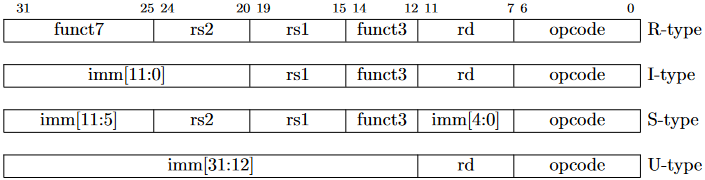
\includegraphics[width=.9\textwidth]{risc-v-formats}

\tiny{Source: The RISC-V Instruction Set Manual, Volume I: Unprivileged ISA,
      Document Version 20191213, page 16}
\end{frame}

\begin{frame}[fragile]{Example 1: RISC-V decoder (1/3)}
\begin{lstlisting}
#define BIT_FIELD(v, e, s) \
    (v >> s) & ((1 << (e - s + 1)) - 1)

static inline int32_t
sign_extend(uint32_t v, int width) {/* ... */};

typedef struct decode {
    uint32_t opcode;
    uint32_t rd;
    uint32_t rs1;
    uint32_t rs2;
    int32_t  imm;
    uint32_t funct3;
    uint32_t funct7;
    /* ... */
} decode_t;
\end{lstlisting}
\end{frame}

\begin{frame}[fragile]{Example 1: RISC-V decoder (2/3)}
\begin{lstlisting}
decode_t
decode(uint32_t raw) {
    uint32_t op = BIT_FIELD(raw, 6, 0);
    switch (type(op)) {
    case I_type:
         return decode_i_type(raw);
    case R_type:
         return decode_r_type(raw);
    /../
    }
}
\end{lstlisting}
\end{frame}

\begin{frame}[fragile]{Example 1: RISC-V decoder (3/3)}
\begin{lstlisting}
decode_t
decode_i_type(uint32_t raw) {
    uint32_t op = BIT_FIELD(raw, 6, 0);
    uint32_t rd = BIT_FIELD(raw, 11, 7);
    uint32_t funct3 = BIT_FIELD(raw, 14, 12);
    uint32_t rs1 = BIT_FIELD(raw, 19, 15);
    int32_t imm = sign_extend(
        BIT_FIELD(raw, 31, 20), 12);

    return (decode_t){.op = op, .rd = rd,
                      .funct3 = funct3, .rs1 = rs1,
                      .imm = imm};
}
\end{lstlisting}
\end{frame}

\begin{frame}{Example 2: Intel\reg~IA-64}
\centering
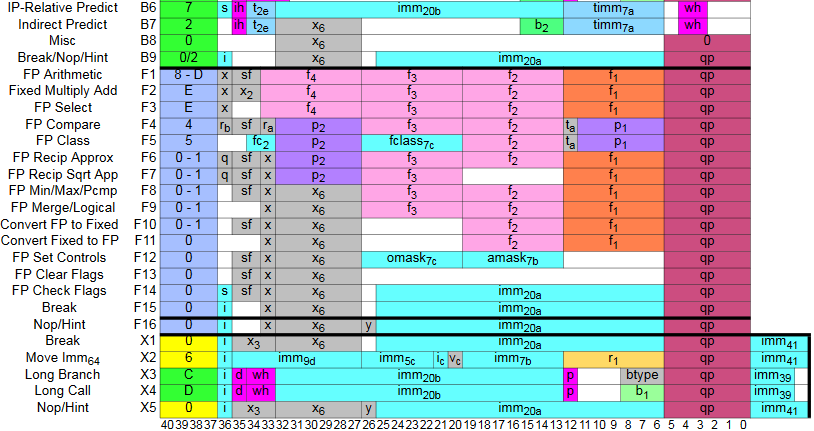
\includegraphics[width=.9\textwidth]{itanium-formats}

\tiny{Source: Intel\reg~Itanium\reg~Architecture Software
      Developer’s Manual, Revision 2.3, page 305}
\end{frame}

\begin{frame}{Example 3: Intel\reg~IA-32}
\centering
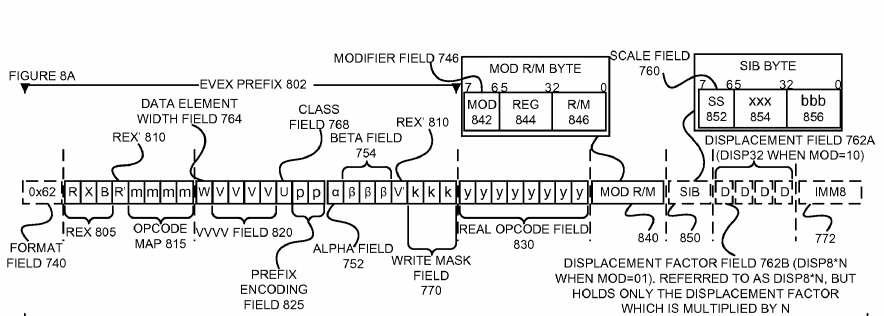
\includegraphics[width=.9\textwidth]{ia32-evex}

\tiny{J.C.S. Adrian et al. Systems, Apparatuses, and Methods for Blending Two
      Source Operands into a Single Destination Using a Writemask. US Patent
      Application Publication. №~2012/0254588 A1}
\end{frame}

\begin{frame}{Что извлекать из машинного кода инструкции}
\begin{centering}
\inputpicture{instruction-anatomy}
\end{centering}

На выходе декодера:
\begin{itemize}
\item Успех, неуспех, недостаточно данных
\item Для успеха: длина инструкции
\item Для успеха: эмулирующая процедура
\end{itemize}
\end{frame}

\begin{frame}{Декодирование}
\begin{itemize}
\item Код декодера редко пишется вручную, он генерируется по описанию:
\item \texttt{\textcolor{red}{A5} \textcolor{blue}{Y}\textcolor{green}{X} 0\textcolor{orange}{Z} 00} $\Rightarrow$ \textcolor{red}{MOD} \textcolor{green}{RX}, \textcolor{blue}{RY}, \textcolor{orange}{RZ}
\item В общем случае: классическаяя задача построения синтаксического анализатора.
\item На практике: специализированные инструменты и языки
\item Пример декодера --- XED (x86 encoder-decoder) \url{https://software.intel.com/sites/landingpage/pintool/docs/61206/Xed/html/}.
\end{itemize}
\end{frame}

\begin{frame}{Декодирование: суровая реальность}
\begin{itemize}
\item Переменная длина инструкций. IA-32: от 8 до 120 бит. Сколько байт пытаться декодировать за один раз?
\item Зависимость смысла от префикса, режима работы процессора. Пример: 0x40–0x4f в IA-32/Intel~64/AMD64
\item Полное несоответствие какому-либо здравому смыслу
\end{itemize}
\end{frame}

\begin{frame}{Дизассемблирование}
\begin{itemize}
\item Дизассемблирование --- перевод инструкций из машинного представление понятный
человеку вид (мнемонику).
\item Закодирование (encoding) --- перевод инструкций из мнемонической записи в
машинный код.
\end{itemize}
\pause
Вопрос: однозначны ли операции: декодирования, дизассемблирования, кодирования?
\end{frame}

\section{Execute}

\begin{frame}{Исполнение}
\begin{itemize}
\item Базовая единица --- функция-эмулятор одной инструкции (service routine).
\item s.r. пишутся на языке высокого уровня --- переносимость кода между хозяйскими
платформами, компиляторами.
\item Используются генераторы кода.
\item Пример: SimGen --- из одного описания генерируются декодер, дизассемблер и s.r.
\end{itemize}
\end{frame}

\begin{frame}[fragile]{Simulated state}
\begin{lstlisting}
typedef struct {
    uint32_t regs[16];
    bool z_flag;
    bool n_flag;
    bool o_flag;
    bool c_flag;
    uint32_t pc;
} cpu_t;
\end{lstlisting}
\end{frame}

\begin{frame}[fragile]{Example: ADD reg reg reg}
\begin{lstlisting}

void add32_rrr(cpu_t *cpu, int src1, int src2, int dst) {
    cpu->regs[dst] = cpu->regs[src1]
                   + cpu->regs[src2];
\end{lstlisting}
\pause

\begin{lstlisting}
    cpu->z_flag = cpu->regs[dst] == 0;
    cpu->n_flag = cpu->regs[dst] & (1 << 31);
    cpu->o_flag = cpu->regs[dst] < 
            MAX(cpu->regs[src1], cpu->regs[src2]);
    cpu->c_flag = calc_c_flag(cpu->regs[src1],
                              cpu->regs[src2]);
}
\end{lstlisting}
\end{frame}

\begin{frame}{Intel\reg~IA-32 CALL}
\centering
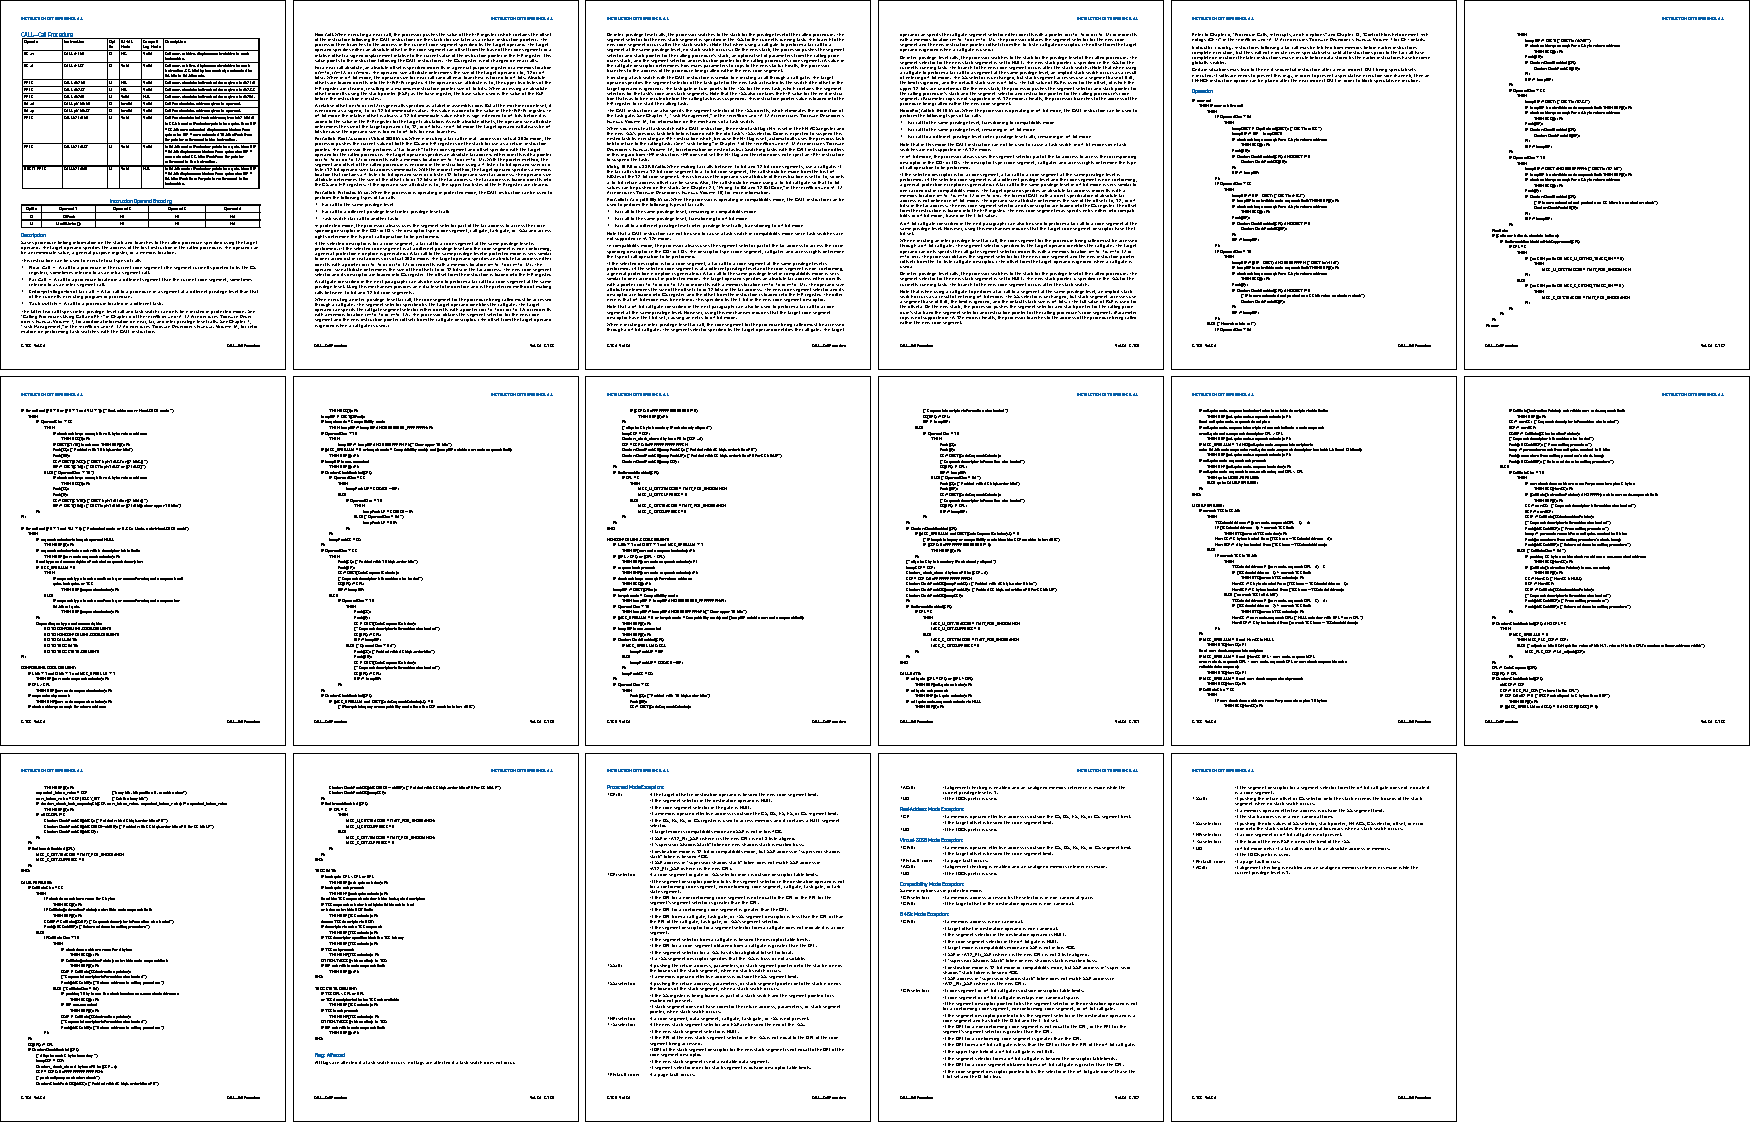
\includegraphics[width=\textwidth]{ia32-call}

\tiny{Source: Intel\reg~64 and IA-32 Architectures Software Developer’s Manual,
      Order Number: 325462-073US, pages 716-732.}
\end{frame}

\section{Write Back}

\begin{frame}{Запись результата в память}

<<Обычная>> запись в память:

\texttt{write_mem(cpu, dst_addr, data, size);}\pause

\pause

\begin{itemize}
    \item Невыровненный адрес,
    \item Граница страниц,
    \item Попытки изменить регион памяти доступный только для чтения,
    \item Часть результата может быть записана, а потом случится исключение.
\end{itemize}

\end{frame}

\section{Exceptions}

\begin{frame}{Уточненный цикл работы}
\centering
\resizebox{9cm}{7cm}{\inputpicture{interp-cycle-expanded-exception}}
\end{frame}

\begin{frame}{Классификация} % TODO a tree diagram?
\begin{itemize}
\item Interruptions (термин из документации IA-64) — вмешательство, перерыв, приостановка
\item Exception — синхронное исключение, без повторения текущей инструкции
\item Fault — синхронное, с повторением текущей инструкции
\item Trap — синхронное, без повторения, намеренно вызванное
\item Interrupt — внешнее асинхронное прерывание
\item Abort — внешние асинхронное с отсутствием информации о точке возврата
\end{itemize}
\end{frame}

\section{Advance \texttt{PC}}

\begin{frame}{Продвижение \texttt{\$PC}}
\begin{itemize}
    \item Для большинства команд увеличение счетчика на длину обработанной инструкции. \\
    Ислючение: \texttt{REP MOVS}.
    \pause\bigskip
    \item Явное изменение \texttt{\$PC} --- команды управления исполнением:
    \begin{itemize}
        \item (Un)conditional (In)direct Jump/Branch,
        \item Call/Return (subroutine).
        \item System call/return.
        \item ...
    \end{itemize}
\end{itemize}
\end{frame}

\section{Улучшенные схемы}

\begin{frame}{Преимущества и недостатки интерпретации}
\begin{itemize}
\item Пишется на языках высокого уровня: код переносим
\item Простая структура: надёжность, расширяемость, переиспользование
\end{itemize}
\pause
\begin{itemize}
\item (Очень) низкая скорость работы
\end{itemize}
\end{frame}

\begin{frame}[fragile]{Куда тратится время?}
\begin{lstlisting}
start: interruption = false;
while (!interruption) {
    raw_code = fetch(PC);
    (opcode, operands) = decode(raw_code); // <-- здесь
    switch (opcode) { // <-- здесь
    case opcode1:
        func1(operands); PC++; break;
    case opcode2:
        func2(operands); PC++; break;
    /*...*/
    }
}
handle_interruption();
goto start;
\end{lstlisting}
\end{frame}

\begin{frame}[fragile]{Шитая интерпретация (threaded interpretation)}
Вместо возвращения к началу цикла «прыгаем» прямо на исполнение следующей инструкции
\begin{lstlisting}
func0: /* simulate instr0 */; PC++;
  next_opcode = decode(fetch(PC));
  goto func_ptr[next_opcode];
func1: /* simulate instr1 */; PC++;
  next_opcode = decode(fetch(PC));
  goto func_ptr[next_opcode];
func2: /* simulate instr2 */; PC++;
  next_opcode = decode(fetch(PC));
  goto func_ptr[next_opcode];
\end{lstlisting}

\tiny\url{http://stackoverflow.com/questions/11227809/why-is-processing-a-sorted-array-faster-than-an-unsorted-array}
\end{frame}

\begin{frame}{Кэширующая интерпретация}
\begin{itemize}
\item В большинстве случаев в код гостевого приложения неизменен
\item Велика вероятность того, что инструкции с некоторыми PC будут исполнены много раз (\textit{задача})
\item Зачем каждый раз их декодировать?
\item Заводим таблицу соответствия «адрес инструкции $\rightarrow$ декодированный результат» 
\end{itemize}

\end{frame}

\begin{frame}[fragile]{Кэширующая интерпретация}
\begin{lstlisting}
while (!interruption) {
  if (operation = cache[PC]); // короткий путь
  else { // не в кэше, длинный путь
  	operation = decode(fetch(PC));
  	cache[PC] = operation; // на будущее
  }
  switch (operation) {
     /* ... */
  }
}
\end{lstlisting}

% \includegraphics[width=0.3\textwidth]{./cached}

\end{frame}

\begin{frame}{Кэширующая интерпретация}
\begin{itemize}
\item Ёмкость любого кэша ограничена, старые данные надо выбрасывать
\item Необходимо следить за неизменностью исходного кода, иначе сохранённое соответствие будет неверным
\end{itemize}
\end{frame}

\section*{Конец}
% The final "thank you" frame 

\begin{frame}{На следующей лекции}
\end{frame}

\begin{frame}

{\huge{Спасибо за внимание!}\par}

\vfill

\tiny{\textit{Замечание}: все торговые марки и логотипы, использованные в данном материале, являются собственностью их владельцев. Представленная здесь точка зрения отражает личное мнение автора, не выступающего от лица какой-либо организации.}

\end{frame}

\end{document}
